\documentclass[aps,prb,superscriptaddress,nofootinbib]{revtex4}
\usepackage{amsfonts}
\usepackage{amsmath}
\usepackage{amssymb}
\usepackage{graphicx}
\usepackage{graphbox}
\usepackage{caption}
\usepackage{bm}
\usepackage{bbm}
\usepackage{cancel}
\usepackage{color}
\usepackage{mathrsfs}
\usepackage[colorlinks,bookmarks=true,citecolor=blue,linkcolor=red,urlcolor=blue]{hyperref}
\usepackage{simpler-wick}
\usepackage{appendix}
\usepackage{float}
\usepackage{sleek-listings}
\usepackage{array}
\usepackage{booktabs}
\setlength{\parindent}{10 pt}
\setlength{\parskip}{2 pt}
\setcounter{MaxMatrixCols}{30}
\bibliographystyle{apsrev}

\newcommand{\normord}[1]{{:\mathrel{#1}:}}
\def\tbs{\textbackslash}
\def \tr{\operatorname{tr}}
\def \Tr{\operatorname{Tr}}


\begin{document}
\title{Quantum Electrodynamics}
\author{Jie Ren}

\FrameTBStyle{mathematica}

\maketitle


\tableofcontents

\section{Introduction}

Quantum electrodynamics (QED) is the field theory for the interaction of charged Dirac field with the U(1) gauge field. 
The Lagrangian is obtained by minimal coupling:
\begin{equation}
	\mathcal{L}_{\mathrm{QED}}
	= \bar\psi \left(i\cancel{D} - m\right)\psi - \frac{1}{4}F_{\mu\nu}F^{\mu\nu}, 
	\quad\text{where}\quad
	\cancel{D} = \gamma^\mu D_\mu 
	= \gamma^\mu [\partial_\mu - i q A_\mu(x)]
	= \cancel{\partial} - iq \cancel{A}.
\end{equation}
The Lagrangian is invariant under the gauge transformation: $\psi(x) \rightarrow e^{iq\alpha(x)}\psi(x)$, $A^\mu(x) \rightarrow A^\mu(x) + \partial^\mu \alpha(x)$, where $q$ is the charge of the field.
For electron, $q=-e$, and for quarks, $q=\frac{2}{3}e$ or $q=-\frac{1}{3}e$.



\subsection{Representations of Lorentz group}
For the $(3+1)$D spacetime, the Lorentz group can be represented as 
\begin{equation}\label{eq:lorentz-parameter}
	\Lambda(\bm \theta,\bm \beta) = \exp\left(i \theta_i J_i +i\beta_i K_i\right), \quad
	\theta_i \equiv \frac{1}{2}\varepsilon_{ijk}\omega_{jk},\quad
	\beta_i \equiv \omega_{i0},
\end{equation}
where the Lie algebra contains 3 rotational generators $J_i \equiv \frac{1}{2}\varepsilon_{ijk}M^{jk}$ and 3 boost generators $K_i \equiv M^{i0}$. 
In the fundamental representation, the generators are represented by
\begin{equation*}
\begin{aligned}
	J_1 &= \left[\begin{array}{cccc} 0 & & & \\ & 0 & & \\ & & 0 & -i \\ & & i & 0 \end{array}\right], & 
	J_2 &= \left[\begin{array}{cccc} 0 & & & \\ & 0 & & i \\ & & 0 & \\ & -i & & 0 \end{array}\right], &
	J_3 &= \left[\begin{array}{cccc} 0 & & & \\ & 0 & -i & \\ & i & 0 & \\ & & & 0 \end{array}\right], \\
	K_1 &= \left[\begin{array}{cccc} 0 & -i & & \\ -i & 0 & & \\ & & 0 & \\ & & & 0 \end{array}\right], & 
	K_2 &= \left[\begin{array}{cccc} 0 & & -i & \\ & 0 & & \\ -i & & 0 & \\ & & & 0 \end{array}\right], &
	K_3 &= \left[\begin{array}{cccc} 0 & & & -i \\ & 0 & & \\ & & 0 & \\ -i & & & 0 \end{array}\right].
\end{aligned}
\end{equation*}
The Lie algebra of the Lorentz algebra can be explicitly done using the fundamental representation. 
The result is
\begin{equation}
	\left[J_i, J_j\right] = i \varepsilon_{ijk} J_k, \quad
	\left[J_i, K_j\right] = i \varepsilon_{ijk} K_k, \quad
	\left[K_i, K_j\right] = -i\varepsilon_{ijk} J_k.
\end{equation}
A special combination of those generators $N_i^{L/R} \equiv \frac{1}{2}(J_i \mp i K_i)$ will create two independent algebras:
\begin{equation}\label{eq:RFT-LG-Alg}
\begin{aligned}
	\left[N_i^L, N_j^L \right] &= i\varepsilon_{ijk}N_k^L, \quad
	\left[N_i^R, N_j^R \right] &= i\varepsilon_{ijk}N_k^R, \quad
	\left[N_i^L, N_j^R \right] &= 0.
\end{aligned}
\end{equation}
In the following, we show such generators give all irreducible representations of the Lorentz group $\mathrm{SO}(3,1)$, which are the building blocks of the relativistic field theory.




We see from (\ref{eq:RFT-LG-Alg}) that after the recombination, the Lorentz algebra breaks into two independent $\mathfrak{su}(2)$ algebra.
Mathematically it means $\mathfrak{so}(3,1) \simeq \mathfrak{su}(2) \oplus \mathfrak{su}(2)$.
That is,
\begin{equation}
	U_{j_L,j_R}(\Lambda)
	= \exp\left[i(\bm\theta+i\bm\beta)\cdot \bm N^L_{j_L} + i(\bm\theta-i\bm\beta)\cdot \bm N^R_{j_R}\right],
\end{equation}
where we see that the representation of the Lorentz algebra can be labeled by $j_L$ and $ j_R$.
In relativistic QFT, the Lorentz symmetry restricts the possible terms that can appear in the Lagrangian.
Different free fields correspond to different representations of the Lorentz algebra, and the Lagrangian should be singlet under the Lorentz transformations.


\paragraph*{Trivial representation.}
The $(j_L,j_R) = (0,0)$ representation corresponds to the scalar field denoted as $\phi(x)$.
Since the field itself is singlet, any polynomial of the field in principle can appear in the theory.
When considering the free theory, we restrict our attention to the quadratic terms, therefore the allowed free theory can only be
\begin{equation*}
	\mathcal L_{\mathrm{KG}} = \frac{1}{2}\partial^\mu \phi \partial_\mu \phi -\frac{m^2}{2}\phi^2 
	\simeq -\frac{1}{2}\phi (\partial^2+m^2) \phi.
\end{equation*}
Besides the field Lagrangian $\mathcal L_{\mathrm{KG}}$, there are more general Lorentz-invariant terms that can be added to the Lagrangian, which describe the interaction of the theory.

\paragraph*{Vector representation.}
If we choose $(j_L=j_R=1/2)$, the field is transformed as a Lorentz vector.
We denote the field as $A^\mu(x)$.
Some possible quadratic forms for the vector field that forms singlets are $A^\mu A_\mu$, $(\partial_\mu A^\mu)^2$, $A^\nu \partial^2 A_\nu$, and $\varepsilon_{\mu\nu\rho\lambda} \partial^\mu A^\nu \partial^\rho A^\lambda$.
For the field theory describing the electromagnetic field, we require the theory to further have gauge symmetry, i.e., invariant under $A^\mu(x) \rightarrow A^\mu(x) + \partial^\mu \alpha(x)$.
The gauge invariant forbids the first term and forces the second and third terms to combine as
\begin{equation*}
	(\partial_\mu A^\mu)^2 - A^\nu \partial^2 A_\nu
	\sim \frac{1}{2}(\partial^\mu A^\nu - \partial^\nu A^\mu)(\partial_\mu A^\nu-\partial_\nu A_\mu)
	\equiv \frac{1}{2} F^{\mu\nu}F_{\mu\nu},
	\quad\text{where}\quad
	F^{\mu\nu}\equiv (\partial^\mu A^\nu - \partial^\nu A^\mu).
\end{equation*}
The Lagrangian describing the electromagnetic field is given by
\begin{equation}
	\mathcal{L}_{\mathrm{Maxwell}} = -\frac{1}{4}F_{\mu\nu}F^{\mu\nu}.
\end{equation}
Note that the fourth term is called the \textit{theta term}, which can be written as a boundary term: $\varepsilon_{\mu\nu\rho\lambda} \partial^\mu A^\nu \partial^\rho A^\lambda
	= \partial^\mu (\varepsilon_{\mu\nu\rho\lambda} A^\nu \partial^\rho A^\lambda)$.


\paragraph*{Spinor representation.}
The spinor representations are those with $j_L=1/2$ or $j_R=1/2$. 
Specifically, we define the left-hand spinor $\psi_L = (\psi_L^1, \psi_L^2)^T$ and right-hand spinor $\psi_R = (\psi_R^1, \psi_R^2)^T$ whose transformations define $\Lambda_L$ and $\Lambda_R$:
\begin{equation}\label{eq:qft-left-right-spinor-rep}
	\Lambda_L(\bm\theta,\bm\beta) = \exp\left(\frac{i}{2}\bm\theta\cdot\bm\sigma-\frac{1}{2}\bm\beta\cdot\bm\sigma \right), \quad
	\Lambda_R(\bm\theta,\bm\beta) = \exp\left(\frac{i}{2}\bm\theta\cdot\bm\sigma+\frac{1}{2}\bm\beta\cdot\bm\sigma \right) = \Lambda_L(\bm \theta, -\bm \beta).
\end{equation}
We can create a ``scalar-like'' object by the inner product of the spinors.
Note that the $\psi_L^\dagger \psi_R$ and $\psi_R^\dagger \psi_L$ are Lorentz invariant objects, while the products of two single-handed spinors like $\psi_L^\dagger \psi_L$ or $\psi_R^\dagger \psi_R$ are not.
However, note that $-i\sigma^2 \psi_L^*$ transforms like a right-handed spinor.\footnote{Using the identity $\sigma^2 \cdot \bm\sigma^* \cdot\sigma^2 = -\bm\sigma$, we have $\sigma^2 \psi_L^*
	\rightarrow \sigma^2 \exp\left(-\frac{i}{2}\bm\theta\cdot\bm\sigma^*-\frac{1}{2}\bm\beta\cdot\bm\sigma^* \right) \sigma^2 \sigma^2 \psi_L^* 
	= \Lambda_L(\bm \theta, -\bm\beta) \sigma^2 \psi_L^*$.}
Thus, the left-hand and right-hand spinor can be interchanged by the action of a ``time reversal'' operation $-i\sigma^2 \mathcal K$ (where $\mathcal K$ is complex conjugation).
The bilinears
\begin{equation*}
	\psi_L \cdot \psi_L \equiv -i\psi_L^T \sigma^2 \psi_L,\quad
	\psi_R \cdot \psi_R \equiv -i\psi_R^T \sigma^2 \psi_R
\end{equation*}
are therefore invariants.
The spinor field theory consists of only the left-hand spinor is called the \textit{Majorana theory}:
\begin{equation}
\begin{aligned}
	\mathcal{L}_{\mathrm{Maj}}
	= i \psi_L^\dagger \bar\sigma^\mu \partial_\mu  \psi_L -m(\psi_L \cdot \psi_L + \psi_L^\dagger \cdot \psi_L^\dagger).
\end{aligned}
\end{equation}
The field theory containing both left-hand and right-hand spinors is called the Dirac theory:
\begin{equation}
	\mathcal{L}_{\mathrm{Dirac}} = \bar\psi \left(i\cancel\partial - m\right)\psi
	\equiv \bar\psi \left(i\gamma^\mu \partial_\mu - m\right)\psi,
\end{equation}
where the Dirac spinor contains left- and right-handed Weyl spinors:
\begin{equation*}
	\psi = \begin{pmatrix}
		\psi_L \\ \psi_R
	\end{pmatrix},\ 
	\bar\psi = \begin{pmatrix}
		\psi_R^\dagger & \psi_L^\dagger
	\end{pmatrix},\ 
	\gamma^\mu = \begin{bmatrix}
		0 & \sigma^\mu \\
		\bar\sigma^\mu & 0
	\end{bmatrix}.
\end{equation*}
We remark that under the Dirac spinor basis, the Lorentz algebra is generated by $M^{\mu\nu} = \frac{i}{4}[\gamma^\mu, \gamma^\nu]$, or 
\begin{equation*}
	J_i = \begin{bmatrix}
		\sigma^i & 0 \\ 0 & -\sigma^i
	\end{bmatrix}, \quad 
	K_i = \frac{i}{2}\begin{bmatrix}
		\sigma^i & 0 \\ 0 & -\sigma^i
	\end{bmatrix},
\end{equation*}
using the familiar parametrization (\ref{eq:lorentz-parameter}).
We can easily check that these matrices obey the transformation property (\ref{eq:qft-left-right-spinor-rep}).

Finally, we note that there is another invariants consisting of Dirac field and the vector gauge field:
\begin{equation}
	\mathcal L_\text{int} = q \bar\psi \gamma^\mu A_\mu \psi,
\end{equation}
which produce the QED Lagrangian $\mathcal{L}_\text{QED} = \mathcal{L}_\text{Dirac} + \mathcal{L}_\text{Maxwell}+\mathcal{L}_\text{int}$.








\section{Scattering}

\subsection{$e^+ e^- \rightarrow \mu^+ \mu^-$}
Consider the scattering process ($e_{p_1} + \bar{e}_{p_2} \rightarrow \mu_{p_3} + \bar{\mu}_{p_4}$). 
To the first order, the amplitude correspond to the simplest tree level diagram.
Using the Feynman rule, this process gives the amplitude
\begin{equation}
	i\mathcal M = (-ie)^2 \bar u(p_3) \gamma^\mu v(p_4) \frac{-i g_{\mu\nu}}{(p_1+p_2)^2} \bar v(p_2) \gamma^\nu u(p_1).
\end{equation}
Use the Mandelstam variables $s=p_1+p_2$, the amplitude is
\begin{equation}
	\mathcal M = \frac{e^2}{s} \left[\bar u(p_3) \gamma^\mu v(p_4) \right] \left[\bar v(p_2) \gamma_\mu u(p_1)\right].
\end{equation}
The complex conjugate of the amplitude is
\begin{equation}
	\mathcal M^\dagger = \frac{e^2}{s} \left[\bar u(p_1) \gamma_\mu v(p_2)\right] \left[\bar v(p_4) \gamma^\mu u(p_3) \right].
\end{equation}
Note that we have use the relation 
\begin{equation}
	(\bar u \gamma^\mu v)^\dagger
	= v^\dagger \gamma^{\mu\dagger} \gamma^0 u 
	= v^\dagger \gamma^0 \gamma^{\mu} u
	= \bar v \gamma^\mu u.
\end{equation}
Therefore,
\begin{equation}
	|\mathcal M|^2 = \frac{e^4}{s^2} \left[\bar v(p_4) \gamma^\mu u(p_3) \right] \left[\bar u(p_3) \gamma^\nu v(p_4) \right] \left[\bar v(p_2) \gamma_\mu u(p_1)\right] \left[\bar u(p_1) \gamma_\nu v(p_2)\right].
\end{equation}
If in the scattering experiment the spins are nor measured, the spin averaged cross section is just the sum of spin indices.
The spin sum can actually simplifies the expression, as it gives the orthogonal relations
\begin{equation}
	\sum_s u(p)_s \bar u_s(p) = \cancel p + m, \quad
	\sum_s v(p)_s \bar v_s(p) = \cancel p - m.
\end{equation}
The spin averaged amplitude is
\begin{equation}
	\frac{1}{4}\sum_{\mathrm{spins}}|\mathcal M|^2 
	= \frac{e^2}{4s^2} \Tr\left[(\cancel p_4 -m_\mu) \gamma^\mu (\cancel{p}_3 + m_\mu) \gamma^\nu \right] \Tr\left[(\cancel p_2-m_e) \gamma_\mu (\cancel p_1 +m_e) \gamma_\nu \right].
\end{equation}
Now we evaluate the gamma traces, using the facts $\Tr[\gamma^\mu \gamma^\nu]=4g^{\mu\nu}$ and $\Tr[\gamma^\mu \gamma^\nu \gamma^\rho \gamma^\sigma] = 4g^{\mu\nu}g^{\rho\sigma}-4g^{\mu\rho}g^{\nu\sigma}+4g^{\mu\sigma}g^{\nu\rho}$.
The first trace is
\begin{equation}
\begin{aligned}
	\Tr\left[(\cancel p_4 -m_\mu) \gamma^\mu (\cancel{p}_3 + m_\mu) \gamma^\nu \right]
	&= \Tr\left[\gamma^\alpha \gamma^\mu \gamma^\beta \gamma^\nu \right] p_{4\alpha} p_{3\beta} - m_\mu^2 \Tr[\gamma^\mu \gamma^\nu] \\
	&= 4 (p_3^\mu p_4^\nu + p_3^\nu p_4^\mu) - 4g^{\mu\nu}(p_3\cdot p_4 + m_\mu^2)
\end{aligned}
\end{equation}
The second is of the same form as the first, we can similarly get
\begin{equation}
	\Tr\left[(\cancel p_2-m_e) \gamma_\mu (\cancel p_1 +m_e) \gamma_\nu \right] 
	= 4 (p_{1\mu} p_{2\nu} + p_{1\nu} p_{2\mu}) - 4g_{\mu\nu}(p_1 \cdot p_2 + m_e^2).
\end{equation}
The final result of the spin average amplitude is
\begin{equation}
	\frac{1}{4}\sum_{\mathrm{spins}}|\mathcal M|^2 
	= \frac{8 e^{4}}{s^{2}}\left(p_{13} p_{24}+p_{14} p_{23}+m_{\mu}^{2} p_{12}+m_{e}^{2} p_{34}+2 m_{e}^{2} m_{\mu}^{2}\right),
\end{equation}
where $p_{ij}\equiv p_i \cdot p_j$.
The amplitude is in a better form with the Mandelstam variables $s$, $t$ and $u$:
\begin{equation}
\begin{aligned}
	s &=\left(p_{1}+p_{2}\right)^{2}=\left(p_{3}+p_{4}\right)^{2}=2 m_{e}^{2}+2 p_{12}=2 m_{\mu}^{2}+2 p_{34}, \\
	t &=\left(p_{1}-p_{3}\right)^{2}=\left(p_{2}-p_{4}\right)^{2}=m_{e}^{2}+m_{\mu}^{2}-2 p_{13}=m_{e}^{2}+m_{\mu}^{2}-2 p_{24}, \\
	u &=\left(p_{1}-p_{4}\right)^{2}=\left(p_{2}-p_{3}\right)^{2}=m_{e}^{2}+m_{\mu}^{2}-2 p_{14}=m_{e}^{2}+m_{\mu}^{2}-2 p_{23} .
\end{aligned}
\end{equation}
Note that $s+t+u = 2 m_e^2 + 2 m_\mu^2$. 
After some algebra, we get
\begin{equation}
	\frac{1}{4} \sum_{\mathrm{spins }}|\mathcal{M}|^{2}=\frac{2 e^{4}}{s^{2}}\left[t^{2}+u^{2}+4 s\left(m_{e}^{2}+m_{\mu}^{2}\right)-2\left(m_{e}^{2}+m_{\mu}^{2}\right)^{2}\right].
\end{equation}




\subsection{$e^- p^+ \rightarrow e^- p^+$}
Next we consider the Rutherford scattering ($e_{p_1} + p_{p_2} \rightarrow e_{p_3} + p_{p_4}$).
This correspond to the same tree-level diagram as ($e_{p_1} + \bar{e}_{p_2} \rightarrow \mu_{p_3} + \bar{\mu}_{p_4}$) except a rotation.
We immediately get the amplitude:
\begin{equation}
	|\mathcal M|^2 = -\frac{e^4}{t^2} \left[\bar u(p_3) \gamma^\mu u(p_1) \right] \left[\bar u(p_1) \gamma^\nu u(p_3) \right] \left[\bar u(p_4) \gamma_\mu u(p_2)\right] \left[\bar u(p_2) \gamma_\nu u(p_4)\right].
\end{equation}
Note that the minus sign comes from the positive charge of proton.
The spin-averaged amplitude is
\begin{equation}
	\frac{1}{4}\sum_{\mathrm{spins}}|\mathcal M|^2 
	= \frac{e^2}{4t^2} 
	\Tr\left[(\cancel p_3 +m_e) \gamma^\mu (\cancel{p}_1 + m_e) \gamma^\nu \right] 
	\Tr\left[(\cancel p_4+m_p) \gamma_\mu (\cancel p_2 +m_p) \gamma_\nu \right].
\end{equation}
The trace is evaluated similarly:
\begin{equation}
\begin{aligned}
	\Tr\left[(\cancel p_3 +m_e) \gamma^\mu (\cancel{p}_1 + m_e) \gamma^\nu \right] 
	&= 4 (p_{1}^{\mu} p_{3}^{\nu} + p_{1}^{\nu} p_{3}^{\mu}) - 4g^{\mu\nu}(p_{13} - m_e^2), \\
	\Tr\left[(\cancel p_4+m_p) \gamma_\mu (\cancel p_2 +m_p) \gamma_\nu \right] 
	&= 4 (p_{2\mu} p_{4\nu} + p_{2\nu} p_{4\mu}) - 4g_{\mu\nu}(p_{24} - m_p^2).
\end{aligned}
\end{equation}
Therefore,
\begin{equation}
	\frac{1}{4}\sum_{\mathrm{spins}}|\mathcal M|^2 
	= \frac{8 e^{4}}{t^{2}}\left(p_{12} p_{34}+p_{14} p_{23} - m_{p}^{2} p_{13} - m_{e}^{2} p_{24}+2 m_{e}^{2} m_{p}^{2}\right).
\end{equation}
The Mandelstam variables are
\begin{equation}
\begin{aligned}
	s &= m_{e}^{2} + m_p^2 + 2 p_{12} = m_e^2 + m_{p}^{2}+2 p_{34}, \\
	t &= 2 m_{e}^{2}-2 p_{13} = 2m_{p}^{2} -2 p_{24}, \\
	u &= m_{e}^{2} + m_p^2 - 2 p_{14} = m_{e}^{2} + m_p^2 - 2 p_{23}.
\end{aligned}
\end{equation}
After some algebra we get
\begin{equation}
	\frac{1}{4} \sum_{\mathrm{spins }}|\mathcal{M}|^{2}=\frac{2 e^{4}}{t^{2}}\left[u^{2}+s^{2}+4 t\left(m_{e}^{2}+m_{p}^{2}\right)-2\left(m_{e}^{2}+m_{p}^{2}\right)^{2}\right].
\end{equation}



\subsection{$\gamma e^- \rightarrow \gamma e^-$}
Next we consider the Compton scattering ($\gamma_{k}+e_{p} \rightarrow \gamma_{k'} + e_{p'}$).
There are two corresponding tree-level diagrams: one is an $s$-process, the other is a $u$-process.
The amplitude for $s$-process is
\begin{equation}
	\mathcal M_s = -\frac{e^2}{s-m_e^2}\epsilon_\mu(k') \bar u(p') \gamma^\mu (\cancel p + \cancel k + m_e) \gamma^\nu u(p) \epsilon_\nu(k),
\end{equation}
and the amplitude for $u$-process is
\begin{equation}
	\mathcal M_u = -\frac{e^2}{u-m_e^2} \epsilon_\mu(k) \bar u(p')\gamma^\mu (\cancel p-\cancel k' +m_e)\gamma^\nu u(p) \epsilon_\nu(k').
\end{equation}
Together, the coherent amplitude is
\begin{equation}
	\mathcal M = e^2 \epsilon_\mu(k')\bar u(p')\left[\frac{ \gamma^\mu (\cancel p + \cancel k + m_e) \gamma^\nu }{s-m_e^2} + \frac{\gamma^\nu (\cancel p-\cancel k' +m_e)\gamma^\mu}{u-m_e^2}\right] u(p) \epsilon_\nu(k).
\end{equation}
The conjugate amplitude is
\begin{equation}
	\mathcal M^\dagger = e^2 \epsilon_\alpha(k)\bar u(p)\left[\frac{\gamma^\alpha (\cancel p + \cancel k + m_e) \gamma^\beta}{s-m_e^2} + \frac{\gamma^\beta (\cancel p-\cancel k' +m_e)\gamma^\alpha}{u-m_e^2}\right] u(p') \epsilon_\beta(k').
\end{equation}
If we do note measure the photon polarization, we can use the polarization averaged result.
The photon polarization sum is
\begin{equation}
	\sum_i \epsilon^i_\mu(k) \epsilon^i_\nu(k) = -g_{\mu\nu} + \frac{1}{2E^2}(p_\mu \bar p_\nu + \bar p_\mu p_\nu).
\end{equation}
The second term does not contribute to the amplitude due to the Ward identity.
We can then simply replace the polarization sum with the metric $-g_{\mu\nu}$.
In this way,
\begin{equation}
	\frac{1}{4}\sum_{\mathrm{s,p}}|\mathcal M_s|^2 = \frac{e^4}{(s-m_e^2)^2} \Tr\left[ (\cancel p_2-m_e) \gamma_\nu (\cancel p_1 + \cancel p_2 + m_e) \gamma_\mu (\cancel p_4+m_e) \gamma^\mu (\cancel p_1 + \cancel p_2 + m_e) \gamma^\nu \right].
\end{equation}


\section{Perturbative Renormalization}
As with the scalar field, the partition function with source is defined as
\begin{equation}
	Z[\bar\eta,\eta,J] = \exp\left\{i\int d^dx \mathcal{L}_{\mathrm{int}}\left[\frac{\delta}{i\delta J},\frac{\delta}{i\delta \eta},\frac{i\delta}{\delta \bar\eta}\right]\right\} Z_0[\bar\eta,\eta,J].
\end{equation}
In the following, we will use the dimensional regularization by default. 
Note that the mass dimensionality for the fermion and gauge field is
\begin{equation*}
	[\psi] = \left[\frac{d-1}{2}\right],\quad
	[A] = \left[\frac{d}{2}-1\right],
\end{equation*}
which lead to the coupling constant $e$ to have the dimension
\begin{equation*}
	[e] = \left[2-\frac{d}{2} \right].
\end{equation*}
When $d=4-\epsilon$, we make the replacement
\begin{equation*}
	e \rightarrow e \tilde{\mu}^{\epsilon/2},
\end{equation*}
so that to make the coupling constant $e$ dimensionless.

The interaction will renormalize the field and coefficients to
\begin{equation}
\begin{aligned}
	\psi &= \sqrt{Z_\psi} \psi_R, & m &= Z_m m_R, \\
	A &= \sqrt{Z_A} A_R, & e &= Z_e e_R.
\end{aligned}
\end{equation}
The renormalized Lagrangian is
\begin{equation}
\begin{aligned}
	\mathcal L 
		&= Z_{\psi} \bar\psi_R(i\gamma^\mu \partial_\mu)\psi_R 
		-Z_m Z_\psi m_R \bar\psi_R\psi_R 
		+ Z_{A} \frac{1}{4} F_{R,\mu\nu}F_R^{\mu\nu} - Z_e Z_\psi \sqrt{Z_A} e_R A_R^\mu \bar\psi_R\gamma^\mu \psi_R \\
		&= \mathcal{L}_0 + \mathcal{L}_{\mathrm{int}} + \mathcal{L}_{\mathrm{ct}}.
\end{aligned}
\end{equation}
The we define the coefficients
\begin{equation}
	\delta_{\psi} = Z_\phi - 1,\quad 
	\delta_{m} = Z_m - 1,\quad 
	\delta_A = Z_A - 1, \quad 
	\delta_1 = Z_e Z_\psi \sqrt{Z_A} - 1.
\end{equation}
The counter term also contribute to the perturbative expansion like the interactions.
The counter terms for the fermion propagator come from the diagram expression:
\begin{equation}
\begin{aligned}
	iG_F^{\mathrm{(ct)}}(p)
	&= 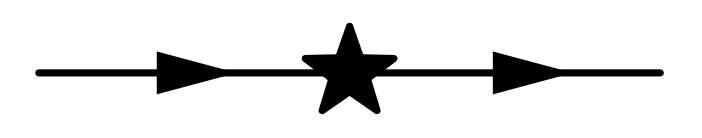
\includegraphics[align=c, width=0.25\linewidth]{pics/QED-ct-1.png} \\
	&= G_F^{(0)}(p) \left[ \delta_{\psi}\cancel{p}-(\delta_m + \delta_\psi) m_R\right] G^{(0)}_F(p) .
\end{aligned}
\end{equation}
The contribution to the electron self energy is
\begin{equation}
	i\Sigma^{(\mathrm{ct})}(p) \equiv \delta_{\psi}\cancel{p}-(\delta_m + \delta_\psi) m_R.
\end{equation}

Similarly, the counter term contribution to the photon self energy is
\begin{equation}
\begin{aligned}
	i \Pi^{(
	\mathrm{ct})}_{\mu\nu}(k) 
	&= 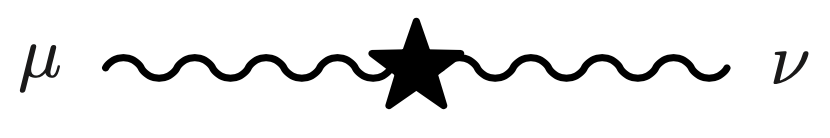
\includegraphics[align=c,width=0.25\linewidth]{pics/QED-ct-2.png} \\
	&= \delta_A [-p^2 g_{\mu\nu} + (1-\xi)p_\mu p_\nu].
\end{aligned}
\end{equation}
In Landau gauge, $\xi=1$ and we can ignore the $p_\mu p_\nu$ terms, and the photon self-energy is always proportional to $g_{\mu\nu}$.
Whenever other gauge choices are concerned, we can simply replace $g_{\mu\nu}$ with
$g_{\mu\nu} - (1-\xi)\frac{p_\mu p_\nu}{p^2}$.

The counter term contribution to the QED vertex is
\begin{equation}
	\Gamma^{\mathrm{(ct)}\mu}_{\alpha\beta} 
	= 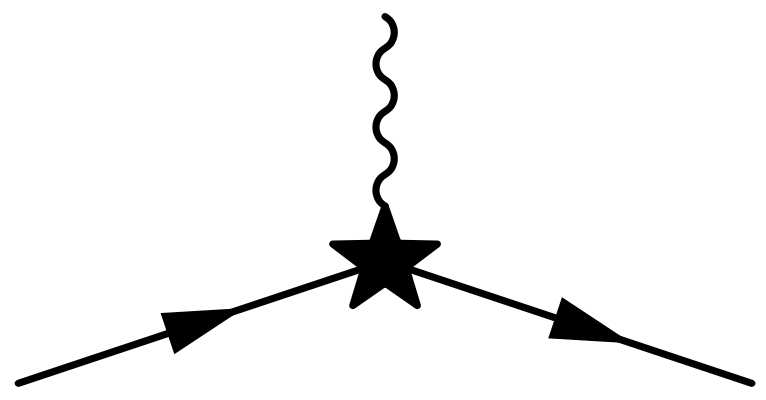
\includegraphics[align=c, width=0.2\linewidth]{pics/QED-ct-3.png} 
	= -\delta_1 \gamma^{\mu}_{\alpha\beta}.
\end{equation}



\subsection{Vacuum Polarization}

Consider the one-loop correction to the photon propagator:
\begin{equation}
\begin{aligned}
	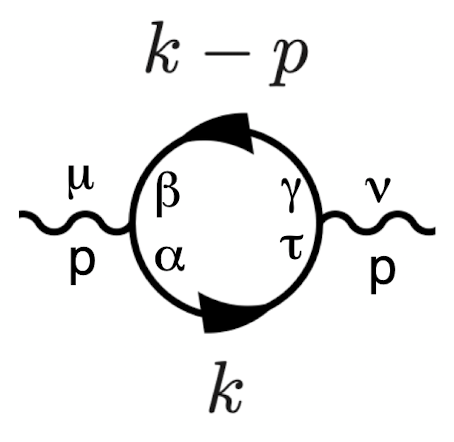
\includegraphics[align=c,width=0.15\linewidth]{pics/QED-2.png} 
	&\simeq (-ie_R)^2\wick{
		A_\mu \c2{\bar\psi}_\alpha \gamma^\mu_{\alpha\beta} \c1{\psi}_\beta 
		A_\nu \c1{\bar\psi}_\gamma \gamma^\nu_{\gamma\tau} \c2{\psi}_\tau
	} \\
	&\equiv iA_\mu \Pi^{\mu\nu}(p) A_\nu.
\end{aligned}
\end{equation}
The self energy is:
\begin{equation}
\begin{aligned}
	i\Pi^{\mu\nu}(p) 
	&= -e_R^2 \int\frac{d^4 k}{(2\pi)^4} \mathrm{Tr}\left[\gamma^\mu G^{(0)}_F(k-p) \gamma^\nu G^{(0)}_F(k) \right] \\
	&= -e_R^2 \int\frac{d^4 k}{(2\pi)^4} 
	\frac{\mathrm{Tr}\left[\gamma^\mu (\cancel k- \cancel p +m_R) \gamma^\nu (\cancel k +m) \right]}{(k^2-m_R^2)[(p-k)^2-m_R^2]}.
\end{aligned}
\end{equation}

The trace of the Dirac matrices can be evaluated in \texttt{Mathematic} using the \texttt{FeynCalc} package:

\begin{lstlisting}[style=mathematicaFrameTB]
(*Dirac trace using FeynCalc`*)
res=DiracTrace[GA[\[Mu]].(GS[k-p]+m).GA[\[Nu]].(GS[k]+m)];
DiracSimplify[res]
\end{lstlisting}

The Dirac trace is:
\begin{equation}
\begin{aligned}
	&\ \mathrm{Tr}\left[\gamma^\mu (\cancel k- \cancel p +m_R) \gamma^\nu (\cancel k +m_R) \right] \\
	=&\ 4 \left[g^{\mu\nu} \left(k\cdot p-{k}^2+m_R^2\right)+ 2k^\mu k^\nu - k^\mu p^\nu - p^\mu k^\nu \right].
\end{aligned}
\end{equation}
Using the Feynman parameters, the denominator is:
\begin{equation}
\begin{aligned}
	\frac{1}{(k^2-m_R^2)[(p-k)^2-m_R^2]}
	&= \frac{1}{\left\{[k-p(1-x)]^2-[m_R^2+p^2 x(x-1)]\right\}^2} \\
	&\equiv \frac{1}{\left\{[k-p(1-x)]^2 - D_x \right\}^2}.
\end{aligned}
\end{equation}
Since the Ward identity requires that the $p^\mu$ term in the propagator do not contribute to any scattering process, we then shift $k \rightarrow k + p(1-x)$ and drop all $p^\mu$ linear term. 
The final result is simplified to:
\begin{equation}
\begin{aligned}
	i\Pi^{\mu \nu}(p) 
	&= -4 e_R^{2} \int_0^1 dx
		\int \frac{d^{4} k}{(2 \pi)^{4}}  \frac{2 k^{\mu} k^{\nu}-g^{\mu \nu}\left[k^{2}-x(1-x) p^{2}-m_R^{2}\right]}{\left[k^{2}-D_x \right]^{2}} \\
	&\simeq 4e_R^2 g^{\mu\nu} \int_0^1 dx \int\frac{d^4 k}{(2 \pi)^{4}}  
		\frac{\frac{1}{2}k^{2}-x(1-x) p^{2}-m_R^{2}}{\left[k^{2}-D_x \right]^{2}} \\
	&\simeq -ie_R^2 g^{\mu\nu} \int_0^1 dx\ \frac{\Omega_d \tilde{\mu}^\varepsilon}{(2\pi)^d} \int_0^\infty dk\ k^{d-1} \frac{\left(4-\frac{2}{d} \right) k^{2}+4x(1-x) p^{2}+4m_R^{2}}{\left[k^{2}+D_x\right]^{2}}.
\end{aligned}
\end{equation}
where we have made the Wick rotation, shifted the dimensionality to $(d=4-\varepsilon)$, and made the substitution (since the self-energy $i\Pi^{\mu\nu} \propto g^{\mu\nu}$):
\begin{equation}
	k^\mu k^\nu \rightarrow \frac{1}{d} k^2 g^{\mu\nu}.
\end{equation}

The remaining problem is to regularize and renormalize the divergent integral
\begin{equation}
	I_\varepsilon(x) \equiv \frac{\Omega_{4-\varepsilon} \tilde{\mu}^\varepsilon}{(2\pi)^{4-\varepsilon}} \int_0^\infty dk\ k^{3-\varepsilon} \frac{\left(4-\frac{8}{4-\varepsilon} \right) k^{2}+4x(1-x) p^{2}+4m_R^{2}}{\left[k^{2}+D_x\right]^{2}}.
\end{equation}

\subsubsection{Regularization and Renormalization}
In $(4-\varepsilon)$-dimensional Euclidean space, the integral is convergent.
The $\varepsilon$-expansion is carried out in \texttt{Mathematica} using the following code:

\begin{lstlisting}[style=mathematicaFrameTB]
omg = (2*Pi^(d/2))/(Gamma[d/2]);
cof = \[Mu]^(4-d)*omg/(2*Pi)^d;
nom = k^(d-1)*((4-8/(4-\[Epsilon]))k^2+4x*(1-x)p^2+4m^2);
int = cof*Integrate[nom/(k^2+D)^2,{k,0,Infinity}][[1]];
map = D->m^2-p^2*x*(1-x);
ans = Series[int/.{d->4-\[Epsilon]},{\[Epsilon],0,0}];
ans /. map // Simplify
\end{lstlisting}

The result is
\begin{equation}
	I_\varepsilon(x) = \frac{p^2 x(1-x)}{2\pi^2} \left[\frac{2}{\varepsilon}+\ln\left(\frac{4\pi e^{-\gamma_E} \tilde\mu^2}{m_R^2-p^2 x(1-x)}\right)\right]
\end{equation}
So the photon self-energy is (also denote $\mu^2=4\pi e^{-\gamma_E} \tilde\mu^2$):
\begin{equation}
	\Pi^{\mu\nu}(p) 
	= -\frac{e_R^2 p^2 g^{\mu\nu}}{6\pi^2 \varepsilon} 
	-\frac{e_R^2 p^2 g^{\mu\nu}}{2\pi^2} \int_0^1 dx\ x(1-x)
	\ln\left[\frac{\mu^2}{m_R^2-p^2 x(1-x)}\right]
\end{equation}
The counter term coefficient can be chosen as
\begin{equation}
	\delta_A = -\frac{e_R^2}{6\pi^2 \epsilon}.
\end{equation}
The renormalized photon self-energy is then
\begin{equation}
\begin{aligned}
	\Pi^{\mu\nu}(p) 
	&= -\frac{e_R^2 p^2 g^{\mu\nu}}{2\pi^2} \int_0^1 dx\ x(1-x)
	\ln\left[\frac{\mu^2}{m_R^2-p^2 x(1-x)}\right] \\
	&= \frac{e_R^2 p^2 g^{\mu\nu}}{2\pi^2} \left\{\frac{1}{3}\ln\left(\frac{m_R}{\mu}\right)
	 + \int_0^{1} dx\ x(1-x) \ln\left[1-\frac{p^2 x(1-x)}{m_R^2}\right] \right\}.
\end{aligned}
\end{equation}


\subsubsection{Physical Observable}

The photon self-energy has the form
\begin{equation}
	\Pi^{\mu\nu}(p) = -e_R^2 \left[g^{\mu\nu}-(1-\xi)p^\mu p^\nu\right] g^{\mu\nu} \Pi_2(p),
\end{equation}
where
\begin{equation}
	\Pi_2(p) = \frac{1}{2\pi^2} \int_0^1 dx\ x(1-x)
	\ln\left[\frac{\mu^2}{m_R^2-p^2 x(1-x)}\right]
\end{equation}
The one-loop correction to photon propagator is
\begin{equation}
\begin{aligned}
	iG^{\mu\nu}_\gamma(p) 
	&= -i \frac{g^{\mu\nu}}{p^2} \left(1 + \sum_{n=1}^\infty (-e_R^2)^n \Pi_2^n(p) \right) \\
	&= -i\frac{g^{\mu\nu}}{p^2 \left[1+e_R^2\Pi_2(p) \right]}.
\end{aligned}
\end{equation}

We can choose the on-shell condition that the photon has no rest mass:
\begin{equation}
	\Pi_2(0) = 0 \quad \Longrightarrow \quad
	\mu = m_R.
\end{equation}
Note that the propagator is related to the Coulomb potential.\footnote{The Coulomb potential arises just like we derive the force (\ref{eq:field-to-force}), but the sources have additional charge $e_R$, and the photon is mass less, so $V(p) = \frac{e_R^2}{p^2}$ for free field.
}
To the second order,
\begin{equation}
\begin{aligned}
	V(p) &= e_R^2 \frac{1-e_R^2 \Pi_2(p)}{p^2} + O(e_R^6) \\
	&= \frac{e_R^2}{p^2}\left\{1 + \frac{e_R^2}{2\pi^2}\int_0^1 dx\ x(1-x)\ln\left[1-\frac{p^2 x(1-x)}{m_R^2}\right] + O(e_R^4)\right\}.
\end{aligned}
\end{equation}

Consider the small momentum limit, where the integral in approximated by
\begin{equation}
\begin{aligned}
	\int_0^1 dx\ x(1-x)\ln\left[1-\frac{p^2 x(1-x)}{m_R^2}\right]
	\approx -\frac{p^2}{m_R^2} \int_0^1 dx\ x^2(1-x)^2 = -\frac{p^2}{30 m_R^2}.
\end{aligned}
\end{equation}
This implies
\begin{equation}
	V(p) = \frac{e_R^2}{p^2} - \frac{e_R^4}{60\pi^2 m_R^2}.
\end{equation}
The Fourier transformation gives
\begin{equation}
	V(r) = -\frac{e_R^2}{4\pi r} - \frac{e_R^4}{60\pi^2 m_R^2}\delta^{(3)}(r).
\end{equation}
For atomic orbit, since only the ($L=0$)-orbit have support at $r=0$, this extra potential will shift the spectrum.
This effect is called the \textit{Lamb shift}.

On the other hand, the the large momentum limit,
\begin{equation}
	V(p) \approx \frac{e_R^2}{p^2}\left[ 1 + \frac{e_R^2}{12\pi^2} \ln \frac{-p^2}{m_R^2} \right],
\end{equation}
which predicts a \textit{Landau pole} beyond which perturbation theory breaks down.




\subsection{One-loop Correction to Electron Propagator}

Consider the one-loop correction to the particle propagator:
\begin{equation}
	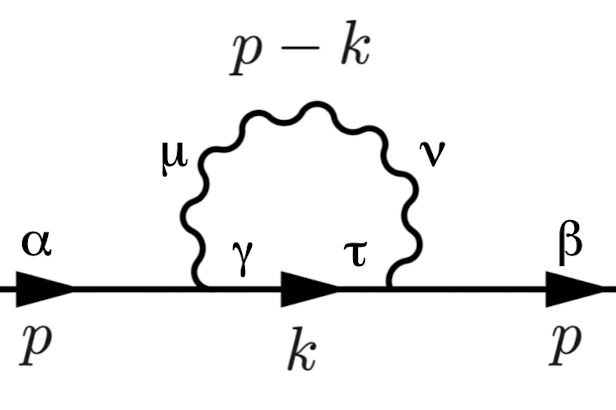
\includegraphics[width=0.2\linewidth,align=c]{pics/QED-1.png} \simeq (-ie_R)^2\wick{
		\c1{A}_\mu \bar\psi_\alpha \gamma^\mu_{\alpha\gamma} \c2{\psi}_\gamma
		\c1{A}_\nu \c2{\bar\psi}_\tau \gamma^\nu_{\tau\beta} \psi_\beta}
	\equiv i\bar\psi_\alpha \Sigma^{\alpha\beta}(p) \psi_\beta.
\end{equation}
The self energy is
\begin{equation}
\begin{aligned}
	i\Sigma_{\alpha\beta}(p)
	&= e_R^2\int\frac{d^4 k}{(2\pi)^4} G^{\mu\nu}_\gamma(p-k) \left[\gamma_\mu G_F(k) \gamma_\nu\right]_{\alpha\beta} \\
	&= -e_R^2\int\frac{d^d k}{(2\pi)^d}\frac{\gamma^\mu(\cancel{k}+m_R)\gamma_\mu}{(p-k)^2(k^2-m_R^2)}.
\end{aligned}
\end{equation}
The seconded equality comes from the contraction:
\begin{equation}
	(-ie)^2\wick{
		\c1{A}_\mu \bar\psi_\alpha \gamma^\mu_{\alpha\gamma} \c2{\psi}_\gamma
		\c1{A}_\nu \c2{\bar\psi}_\tau \gamma^\nu_{\tau\beta} \psi_\beta}
\end{equation}
The nominator can be simplified using the Dirac matrix identities:
\begin{equation}
	\gamma^\mu \gamma_\mu = d, \quad
	\gamma^\mu \gamma^\nu \gamma_\mu = (2-d) \gamma^\nu
	\quad \Longrightarrow \quad
	\gamma^\mu(\cancel{k}+m_R)\gamma_\mu = d m_R+(2-d)\cancel{k}.
\end{equation}
The denominator can be simplify using the Feynman parameter:
\begin{equation}
\begin{aligned}
	\frac{1}{(p-k)^2(k^2-m_R^2)} 
	&= \int_0^1 \frac{dx}{\left[(k-px)^2-(1-x)(m_R^2-p^2 x)\right]^2} \\
	&\rightarrow \int_0^1 \frac{dx}{\left(k^2-D_x\right)^2}
\end{aligned}
\end{equation}
where we have shifted $k \rightarrow k + px$ (note this shift also change the numerator).

The self energy becomes (including a $\tilde \mu$ mass scale):
\begin{equation}
\begin{aligned}
	i\Sigma(p)
	&= e_R^2\tilde{\mu}^{\varepsilon} 
		\int_0^1 [(2-\varepsilon)x\cancel{p}-(4-\varepsilon)m_R] dx 
		\int \frac{d^d k}{(2\pi)^d} 
		\frac{1}{(k^2-D_x)^2} \\
	&= ie_R^2 \int_0^1 dx\ [(2-\varepsilon)x\cancel{p}-(4-\varepsilon)m_R]\ 
		\frac{\tilde{\mu}^{\varepsilon}\Omega_d}{(2\pi)^d} 
		\int \frac{k^{d-1} dk}{(k^2+D_x)^2}.
\end{aligned}
\end{equation}


\subsubsection{Regularization and Renormalization}

The regularization procedure is carried out by the following code:

\begin{lstlisting}[style=mathematicaFrameTB]
omg=(2*Pi^(d/2))/(Gamma[d/2]);
cof=\[Mu]^(4-d)*omg/(2*Pi)^d;
int=cof*Integrate[q^(d-1)/(q^2+D)^2,{q,0,Infinity}][[1]];
map={e->Sqrt[4*Pi*\[Alpha]],EulerGamma->Subscript[\[Gamma],E]};
ans=Series[int/.{d->4-\[Epsilon]},{\[Epsilon],0,0}];
ans/.map//Simplify
\end{lstlisting}

The result is ($\mu^2 = 4\pi e^{-\gamma_E} \tilde\mu^2$)
\begin{equation}
\begin{aligned}
	\Sigma(p) 
	&= \frac{e_R^2}{16\pi^2}\int_0^1 dx \left[(2-\varepsilon)x\cancel{p}-(4-\varepsilon)m_R \right] 
	\left[\frac{2}{\varepsilon}+\ln\frac{\mu^2}{(1-x)(m_R^2-p^2 x)}\right] \\
	&= \frac{e_R^2}{16\pi^2} \left\{ \int_0^1 dx \left[2x\cancel{p}-4m_R \right] 
	\left[\frac{2}{\varepsilon}+\ln\frac{\mu^2}{(1-x)(m_R^2-p^2 x)}\right]-\cancel p + 2m_R\right\}.
\end{aligned}
\end{equation}
The infinity comes from
\begin{equation}
	\frac{e_R^2}{4\pi^2\varepsilon}\int_0^1 dx(x\cancel{p}-2m_R)
	= \frac{e_R^2}{8\pi^2\varepsilon}\cancel{p} - \frac{e_R^2}{2\pi^2\varepsilon}m_R.
\end{equation}
Using the $\overline{\mathrm{MS}}$ subtraction scheme, we choose
\begin{equation}
	\delta_{\psi} = -\frac{e_R^2}{8\pi^2\varepsilon},\quad
	\delta_m = -\frac{3 e_R^2}{8\pi^2\varepsilon},
\end{equation}
and the self energy is
\begin{equation}
	\Sigma(p) 
	= \frac{e_R^2}{16\pi^2} \left\{\int_0^1 dx(2x\cancel{p}-4m_R)\ln\left[\frac{\mu^2}{(1-x)(m_R^2-p^2 x)}\right]-\cancel p + 2m_R \right\}.
\end{equation}


\subsubsection{Physical Observables}

The Dyson series gives:
\begin{equation}
	iG_F(p) = \frac{i}{\cancel p - m_R + \Sigma(p)}
\end{equation}
Experimentally, for a given 
The on-shell subtraction requires that the $m_R$ equals to the physical mass:
\begin{equation}
	\left. \Sigma(\cancel p) \right|_{\cancel p=m_R} = 0, \quad 
	\left. \frac{d}{d \cancel p}\Sigma(\cancel p) \right|_{\cancel p=m_R} = 0.
\end{equation}
To implement the on-shell condition, we have to modify the subtraction scheme to
\begin{equation}
\begin{aligned}
	\delta_{\psi} &= -\frac{e_R^2}{8\pi^2}\left(\frac{1}{\varepsilon}+\ln\frac{\mu}{m_R} +A\right), \\
	\delta_m &= -\frac{e_R^2}{8\pi^2}\left(\frac{3}{\varepsilon} + 3\ln\frac{\mu}{m_R} + B\right),
\end{aligned}
\end{equation}
and the self energy is
\begin{equation}
\begin{aligned}
	\Sigma(\cancel p)
	=&\ -\frac{e_R^2}{8\pi^2} \int_0^1 dx(x\cancel{p}-2m_R)\ln\left[(1-x)\left(1- \frac{p^2}{m_R^2} x \right)\right]\\
	&\  -\frac{e_R^2}{8\pi^2} \left[\left(A+\frac{1}{2}\right)\cancel p - (A+B+1)m_R\right].
\end{aligned}
\end{equation}
The first condition
\begin{equation}
\begin{aligned}
	\left. \Sigma(\cancel p) \right|_{\cancel p=m_R}
	&= -\frac{e_R^2}{8\pi^2} m_R \left[\int_0^1 dx\ (x-2) \ln(1-x)^2 - B-\frac{1}{2}\right] \\
	&= -\frac{e_R^2}{8\pi^2} m_R \left(2 - B\right) = 0
\end{aligned}
\end{equation}
gives the mass renormalization coefficient
\begin{equation}
	\delta_m = -\frac{e_R^2}{8\pi^2}\left(\frac{3}{\varepsilon} + 3\ln\frac{\mu}{m_R} + 2\right).
\end{equation}
While in the derivative of the self-energy:
\begin{equation}
	\frac{d}{d \cancel p}\Sigma(m_R)  
	= -\frac{e_R^2}{8\pi^2} \left\{\int_0^1 dx\ \left[ x\ln(1-x)^2 -\frac{2x(x-2)}{1-x}\ln(1-x)\right] + A + \frac{1}{2}\right\},
\end{equation}
there is a divergent integral:
\begin{equation}
	\int_0^1 dx\ \frac{2x(x-2)}{1-x}\ln(1-x),
\end{equation}
indicating an IR divergence.
We can never the less get rid of it by introducing a small mass $m_\gamma$ for photon (which will be set to zero).
This mass term change the denominator in the loop integral:
\begin{equation}
	\frac{1}{\left[(p-k)^2-m_\gamma^2\right](k^2-m_R^2)} 
	= \int_0^1 \frac{dx}{\left[(k-px)^2-D_x -x m_\gamma^2\right]^2}.
\end{equation}
Most derivation remains the same, we just need to make a substitution in the finial result:
\begin{equation}
	D_x \rightarrow D_x + x m_\gamma^2.
\end{equation}
Especially, the introducing of the photon mass will not change the result of the mass renormalization factor we have computed.

The modified self-energy is then
\begin{equation}
\begin{aligned}
	\Sigma(\cancel p)
	=&\ -\frac{e_R^2}{8\pi^2} \int_0^1 dx(x\cancel{p}-2m_R)\ln\left[(1-x)\left(1- \frac{p^2}{m_R^2} x \right) + x \frac{m_\gamma^2}{m_R^2} \right]\\
	&\  -\frac{e_R^2}{8\pi^2} \left[\left(A+\frac{1}{2}\right)\cancel p - (A+B+1)m_R\right].
\end{aligned}
\end{equation}
The derivative is now
\begin{equation}
	\frac{d}{d \cancel p}\Sigma(m_R)  
	= -\frac{e_R^2}{8\pi^2} \left\{ \int_0^1 dx\ \left[ x\ln(1-x)^2 +\frac{2x(2-x)(1-x)}{(1-x)^2 + x \frac{m_\gamma^2}{m_R^2}} \right] + A + \frac{1}{2}\right\},
\end{equation}
Note that in the ($m_\gamma \rightarrow 0$) limit, the asymptotic behavior of the originally divergent integral is
\begin{equation}
	\lim_{m_\gamma \rightarrow 0} \int_0^1 dx\ \frac{2x(2-x)(1-x)}{(1-x)^2 + x \frac{m_\gamma^2}{m_R^2}}
	= -1 - 2\ln \frac{m_\gamma}{m_R}.
\end{equation}
So the second subtraction condition is:
\begin{equation}
	\frac{d}{d \cancel p}\Sigma(m_R)  
	= -\frac{e_R^2}{8\pi^2} \left(A -2 - 2\frac{m_\gamma}{m_R} \right) = 0.
\end{equation}
The field strength renormalization is
\begin{equation}
	\delta_\psi = -\frac{e_R^2}{8\pi^2}\left(\frac{1}{\varepsilon}+\ln\frac{\mu}{m_R} +2+2\ln\frac{m_\gamma}{m_R}\right).
\end{equation}
The final self energy is (shall take the $m_\gamma \rightarrow 0$ limit):
\begin{equation}
\begin{aligned}
	\Sigma(\cancel p)
	=&\ -\frac{e_R^2}{16\pi^2} \int_0^1 dx(2x\cancel{p}-4m_R)\ln\left[(1-x)\left(1- \frac{p^2}{m_R^2} x \right) + 2x \ln\frac{m_\gamma}{m_R} \right]\\
	&\  -\frac{e_R^2}{16\pi^2} \left[\left(5+4\ln\frac{m_\gamma}{m_R}\right)\cancel p - \left(10 +4\ln\frac{m_\gamma}{m_R}\right)m_R\right].
\end{aligned}
\end{equation}



\subsection{One-loop Correction to Vertex}
Consider the one-loop correction to interaction:
\begin{equation}
\begin{aligned}
	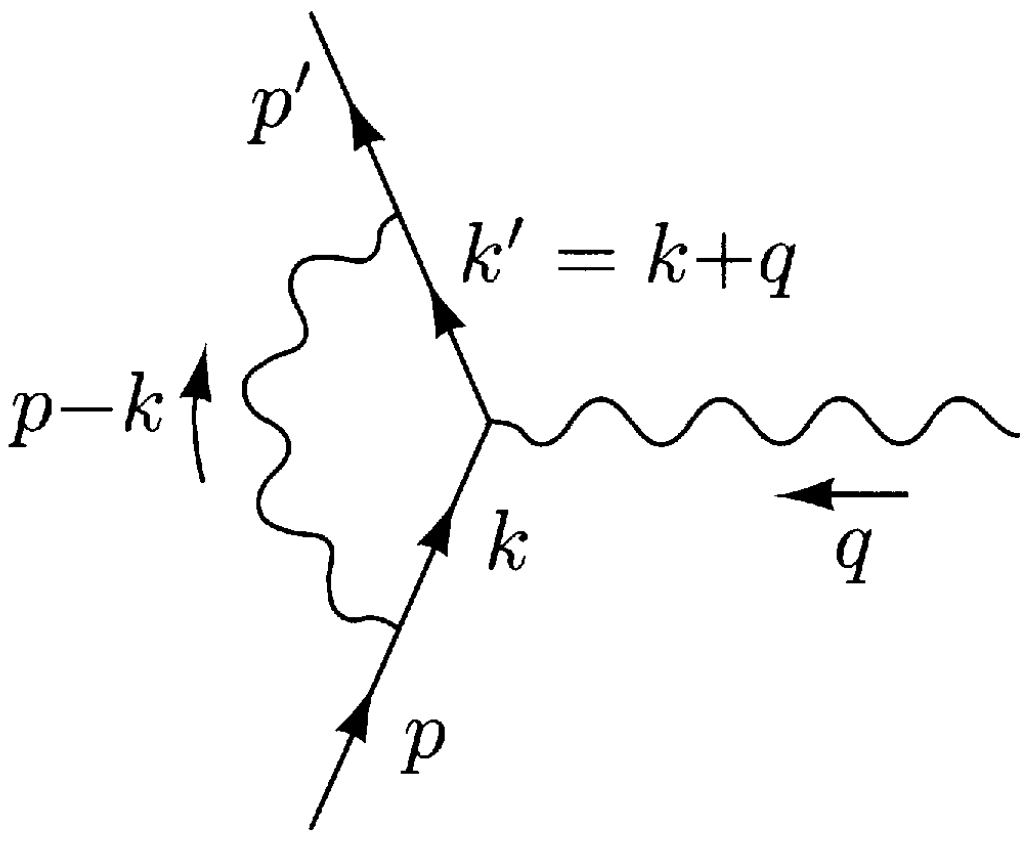
\includegraphics[align=c,width=0.23\linewidth]{pics/QED-3.png}
	& \simeq (-ie_R)^3\wick{
		\c1{A}_\nu \bar\psi_\alpha \gamma^\nu_{\alpha\beta} \c2{\psi}_\beta 
		A_\mu \c2{\bar\psi}_\lambda \gamma^\mu_{\lambda\tau} \c3{\psi}_\tau
		\c1{A}_\xi \c3{\bar\psi}_\rho \gamma^\nu_{\rho\sigma} \psi_\sigma
	} \\ &\equiv -ie A_\mu \Gamma^\mu_{\alpha\beta}(q,p,p') \bar\psi_\alpha \psi_\beta.
\end{aligned}
\end{equation}
The vertex function is:
\begin{equation}
\begin{aligned}
	i\Gamma^\mu_{\alpha\beta}(q,p,p')
	&= -e_R^2 \int\frac{d^4 k}{(2\pi)^4} 
	G_\gamma^{\nu\lambda}(p-k) 
	[\gamma_\nu G_F(k') \gamma^\mu G_F(k) \gamma_\lambda]_{\alpha\beta} \\
	&= e_R^2 \int\frac{d^4 k}{(2\pi)^4} 
	\frac{[\gamma^\nu(\cancel{k}'+m_R)\gamma^\mu (\cancel{k}+m_R)\gamma_\nu]_{\alpha\beta}}{(k^2-m_R^2)(k'^2-m_R^2)(p-k)^2}
\end{aligned}
	\label{eq:QED-loop-vertex}
\end{equation}
Using the following code
\begin{lstlisting}[style=mathematicaFrameTB]
(*numerator*)
den=Contract[GA[\[Nu]].(GS[kp]+m).GA[\[Mu]].(GS[k]+m).GA[\[Nu]]];
DiracSimplify[den]

(*Feynman parameter*)
A1=k^2-m^2;
A2=(k+q)^2-m^2;
A3=(p-k)^2;
{c,b,a}=CoefficientList[x*A1+y*A2+z*A3,{k}];
-b/2//Simplify
-c+b^2/4//Simplify
\end{lstlisting}
The numerator is
\begin{equation}
	-2\cancel{k}\gamma^\mu\cancel{k}'-2m_R^2\gamma^\mu + 4m_R(k + k')^\mu.
\end{equation}
The denominator is
\begin{equation}
	\int \frac{dF_3}{[(k+yq-zp)^2-D_{xyz}]^3},
\end{equation}
where 
\begin{equation*}
\begin{aligned}
	D_{xyz} &= (x+y)m^2 - z(1-z)p^2- y(1-y)q^2-2yzpq \\
	&=(x+y)m_R^2 - xy q^2- yz p'^2 - xz p^2.
\end{aligned}
\end{equation*}
Shift $k^\mu \rightarrow k^\mu + z q_1^\mu - y p^\mu$, throw away all terms with linear $k^\mu$, and replace $k^\mu k^\nu$ with $\frac{1}{d}k^2 g^{\mu\nu}$, the result is
\begin{equation*}
	\frac{4}{d}k^2\gamma^\mu  -2(-y \cancel{q}+z \cancel{p}) \gamma^{\mu}[(1-y) \cancel q+z \cancel p] +4 m_R^{2} \gamma^{\mu}-2 m_R\left[(1-2 y) q^{\mu}+2 z p^{\mu}\right].
\end{equation*}
Note that only the quadratic term is divergent. 
\begin{equation*}
	\Gamma^\mu(p,q_1,q_2) = -i\frac{4e^2\tilde{\mu}^{\epsilon} \gamma^\mu}{d}  \int dF_3 \int \frac{d^dk}{(2\pi)^d} \frac{k^2}{(k^2-D)^3} + \delta\Gamma^\mu(p,q_1,q_2).
\end{equation*}
where $\delta \Gamma^\mu$ stores all the finite part
\begin{equation*}
\begin{aligned}
	& \delta\Gamma^\mu(p,q_1,q_2) \\
	=& \int \frac{e^2 k^3 dk dF_3}{(2\pi)^2(k^2+D)^3} \left\{(-y \cancel{q}+z \cancel{p}) \gamma^{\mu}[(1-y) \cancel q+z \cancel p] -2 m_R^{2} \gamma^{\mu}+ m_R\left[(1-2 y) q^{\mu}+2 z p^{\mu}\right]\right\}.
\end{aligned}
\end{equation*}
The divergent part is
\begin{equation}
	\frac{4 e^2\tilde{\mu}^{\epsilon} \Omega_d \gamma^\mu}{d(2\pi)^d}\int dF_3 \int \frac{k^{d+1}dk}{(k^2+D)^3}
	= \frac{e_R^2}{16\pi^2} \gamma^\mu \int dF_3 \left(\frac{2}{\epsilon}+\ln\frac{\mu^2}{D_{xyz}}\right).
\end{equation}
Using the $\overline{\mathrm{MS}}$ scheme, the coefficient of the counter term is
\begin{equation}
	\delta_e = -\frac{e_R^2}{8\pi^2\varepsilon}.
\end{equation}



\section{Systematic Renormalization}



\subsection{Renormalization Group}
In summery, the renormalization factors are
\begin{equation}
\begin{aligned}
	Z_\psi &= 1 -\frac{e_R^2}{8\pi^2\epsilon} + O(e_R^3), \\
	Z_A &= 1 - \frac{e_R^2}{6\pi^2 \epsilon} + O(e_R^3), \\
	Z_m &= 1 - \frac{e_R^2}{2\pi^2\epsilon} + O(e_R^3), \\
	Z_e &= 1 - \frac{e_R^2}{8\pi^2\epsilon} + O(e_R^3),
\end{aligned}
\end{equation}
which means
\begin{equation}
\begin{aligned}
	\frac{d\ln Z_\phi}{d e_R} &= -\frac{e_R}{4\pi^2 \epsilon} + O(e_R^2), \\
	\frac{d\ln Z_A}{d e_R} &= -\frac{e_R}{3\pi^2 \epsilon} + O(e_R^2), \\
	\frac{d\ln Z_m}{d e_R} &= -\frac{e_R}{\pi^2 \epsilon} + O(e_R^2), \\
	\frac{d\ln Z_e}{d e_R} &= -\frac{e_R}{4\pi^2 \epsilon} + O(e_R^2).
\end{aligned}
\end{equation}
The bare parameters are
\begin{equation}
\begin{aligned}
	\psi_0 &= Z_\psi^{1/2}\psi_R, \\
	A_0 &= Z_A^{1/2} A_R, \\
	m_0 &= Z_m Z_\psi^{-1} m_R, \\
	e_0 &= Z_e Z_\psi^{-1} Z_A^{-1/2} e_R \tilde{\mu}^{\epsilon/2}. 
\end{aligned}
\end{equation}
The RG equation for $e_0$ is
\begin{equation}
	\frac{d\ln e_0}{d\ln \mu}
	= \left(\frac{\ln Z_e}{d e_R} - \frac{\ln Z_\psi}{d e_R} - \frac{1}{2} \frac{\ln Z_A}{d e_R} + \frac{1}{e_R} \right)\frac{de_R}{d\ln \mu} + \frac{\epsilon}{2} = 0.
\end{equation}
The beta function is
\begin{equation}
	\beta(e_R) = \frac{de_R}{d\ln \mu} = -\frac{\epsilon}{2}e_R + \frac{e_R^3}{12\pi^2} + O(e_R^4).
\end{equation}
The RG equation for $m_0$ is
\begin{equation}
	\frac{d\ln m_0}{d\ln \mu}
	= \left(\frac{\ln Z_m}{d e_R} - \frac{\ln Z_\psi}{d e_R}\right)\frac{de_R}{d\ln \mu} + + \frac{1}{m_R}\frac{d m_R}{d\ln\mu} = 0.
\end{equation}
The anomalous dimension of mass is
\begin{equation}
	\gamma_m = \frac{d \ln m_R}{d\ln\mu} = -\frac{3e_R^2}{8\pi^2} + O(e_R^3).
\end{equation}





\end{document}


